% !TeX program = xelatex
\documentclass{article}
\usepackage{kotex}
\usepackage[a4paper,left=3cm, right=3cm, top=2cm, bottom=2cm]{geometry}
\usepackage{amsmath}
\usepackage{graphicx}
\usepackage{caption}
\usepackage{setspace}
\usepackage{xcolor}
\usepackage{titlesec}
\usepackage{amssymb}
\usepackage{tcolorbox}
\usepackage{amsthm}
\usepackage{multirow}
\usepackage{array}
\usepackage{booktabs}
\usepackage{tikz}
\usetikzlibrary{positioning,arrows.meta,calc,shapes.geometric,matrix}
\usepackage{cancel}
\usepackage{pgfplots}
\pgfplotsset{compat=1.18}

\title{8.5 Similarity}
\date{}
\author{}
\setstretch{1.3}

\titleformat{name=\section, numberless}
  {\normalfont\large\bfseries\color{blue}}{}
  {0pt}{}
\geometry{a4paper, margin=1in}

\newcommand{\redheading}[1]{{\vspace{2mm}\noindent\Large\bfseries\color{red!55!black} #1\par}\vspace{2mm}}

\begin{document}
\maketitle

{\itshape\color{blue!45!black}
The matrix for a linear operator $T : V \to V$ depends on the basis selected for $V$.
One of the fundamental problems of linear algebra is to choose a basis for $V$ that makes
the matrix for $T$ as simple as possible---a diagonal or a triangular matrix, for example.
In this section we study this problem.\par}

\vspace{2mm}

\redheading{Simple Matrices for Linear Operators}

Standard bases do not necessarily produce the simplest matrices. Consider $T : R^2 \to R^2$
whose matrix relative to the standard basis $B = \{\mathbf{e}_1, \mathbf{e}_2\}$ is
\begin{equation}
  [T]_B = \begin{bmatrix}1 & 1\\-2 & 4\end{bmatrix} \tag{1}
\end{equation}
Compare this with $[T]_{B'}$ for the same operator $T$ but relative to the basis
$B' = \{\mathbf{u}'_1, \mathbf{u}'_2\}$, where
\begin{equation}
  \mathbf{u}'_1 = \begin{bmatrix}1\\1\end{bmatrix}, \qquad
  \mathbf{u}'_2 = \begin{bmatrix}1\\2\end{bmatrix} \tag{2}
\end{equation}
Since
\[
  T(\mathbf{u}'_1) = \begin{bmatrix}1&1\\-2&4\end{bmatrix}\begin{bmatrix}1\\1\end{bmatrix}
  = \begin{bmatrix}2\\2\end{bmatrix} = 2\mathbf{u}'_1 \qquad\text{and}\qquad
  T(\mathbf{u}'_2) = \begin{bmatrix}1&1\\-2&4\end{bmatrix}\begin{bmatrix}1\\2\end{bmatrix}
  = \begin{bmatrix}3\\6\end{bmatrix} = 3\mathbf{u}'_2
\]
it follows that $[T(\mathbf{u}'_1)]_{B'} = [2,0]^T$ and $[T(\mathbf{u}'_2)]_{B'} = [0,3]^T$, so
\[
  [T]_{B'} = \bigl[\,T(\mathbf{u}'_1)_{B'}\mid T(\mathbf{u}'_2)_{B'}\,\bigr]
  = \begin{bmatrix}2&0\\0&3\end{bmatrix}
\]
This diagonal matrix is simpler than $[T]_B$ and conveys immediately that $T$ scales
$\mathbf{u}'_1$ by a factor of 2 and $\mathbf{u}'_2$ by a factor of 3---information
not evident from $[T]_B$.

The strategy for finding the simplest possible matrix for $T : V \to V$ is to compute
$[T]_B$ for any convenient basis, then change the basis to simplify. Before pursuing this,
we revisit transition matrices.

\vspace{2mm}
\redheading{A New View of Transition Matrices}

Recall from Section~4.7: if $B = \{\mathbf{u}_1, \ldots, \mathbf{u}_n\}$ and
$B' = \{\mathbf{u}'_1, \ldots, \mathbf{u}'_n\}$ are bases for $V$, the transition
matrices are
\begin{equation}
  P_{B\to B'} = \bigl[\,[\mathbf{u}_1]_{B'}\mid[\mathbf{u}_2]_{B'}\mid\cdots\mid
  [\mathbf{u}_n]_{B'}\,\bigr] \tag{3}
\end{equation}
\begin{equation}
  P_{B'\to B} = \bigl[\,[\mathbf{u}'_1]_B\mid[\mathbf{u}'_2]_B\mid\cdots\mid
  [\mathbf{u}'_n]_B\,\bigr] \tag{4}
\end{equation}
where $P_{B\to B'}$ and $P_{B'\to B}$ are inverses of each other. Also, for any
$\mathbf{v} \in V$:
\begin{equation}
  P_{B\to B'}[\mathbf{v}]_B = [\mathbf{v}]_{B'} \tag{5}
\end{equation}
\begin{equation}
  P_{B'\to B}[\mathbf{v}]_{B'} = [\mathbf{v}]_B \tag{6}
\end{equation}
The following theorem shows that these transition matrices can be viewed as matrices for
the identity operator.

\begin{tcolorbox}[colback=red!4, colframe=red!60!black,
  title={\textbf{Theorem 8.5.1}}, boxrule=0.5mm, arc=3mm]
If $B$ and $B'$ are bases for a finite-dimensional vector space $V$, and if $I : V \to V$
is the identity operator on $V$, then
\[
  P_{B\to B'} = [I]_{B',B} \qquad\text{and}\qquad P_{B'\to B} = [I]_{B,B'}
\]
\end{tcolorbox}

\textit{Proof.} Using Formula~(4) of Section~8.4:
\begin{align*}
  [I]_{B',B} &= \bigl[\,[I(\mathbf{u}_1)]_{B'}\mid[I(\mathbf{u}_2)]_{B'}\mid\cdots
  \mid[I(\mathbf{u}_n)]_{B'}\,\bigr]\\
  &= \bigl[\,[\mathbf{u}_1]_{B'}\mid[\mathbf{u}_2]_{B'}\mid\cdots
  \mid[\mathbf{u}_n]_{B'}\,\bigr] = P_{B\to B'} \quad\text{[Formula (3)]}
\end{align*}
The proof that $[I]_{B,B'} = P_{B'\to B}$ is similar. $\blacksquare$

\vspace{2mm}
\redheading{Effect of Changing Bases on Matrices of Linear Operators}

\begin{tcolorbox}[colback=blue!4, colframe=blue!55!black,
  title={\textbf{Problem}}, boxrule=0.5mm, arc=3mm]
If $B$ and $B'$ are two bases for a finite-dimensional vector space $V$, and
$T : V \to V$ is a linear operator, what relationship exists between $[T]_B$ and $[T]_{B'}$?
\end{tcolorbox}

The answer is obtained by writing $T = I \circ T \circ I$ and assigning basis $B'$ to the
first and last copies of $V$, and basis $B$ to the two middle copies, as shown below.

\begin{figure}[ht]
\centering
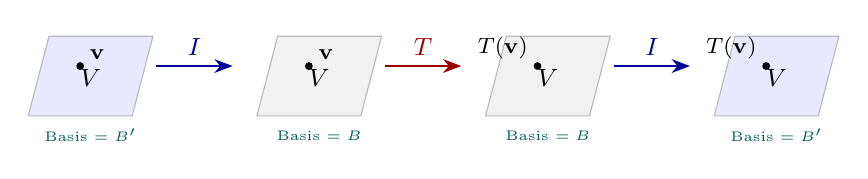
\begin{tikzpicture}[>=Stealth, scale=0.88]
  \foreach \x/\col in {0/blue!9, 3.3/gray!11, 6.6/gray!11, 9.9/blue!9} {
    \fill[\col, draw=gray!55]
      (\x-0.75,0) -- (\x+0.75,0) -- (\x+1.05,1.15) -- (\x-0.45,1.15) -- cycle;
  }
  \node[font=\small] at (0.15,0.55)   {$V$};
  \node[font=\small] at (3.45,0.55)  {$V$};
  \node[font=\small] at (6.75,0.55)  {$V$};
  \node[font=\small] at (10.05,0.55) {$V$};
  \node[font=\tiny, teal!70!black] at (0.15,-0.28)   {Basis $= B'$};
  \node[font=\tiny, teal!70!black] at (3.45,-0.28)  {Basis $= B$};
  \node[font=\tiny, teal!70!black] at (6.75,-0.28)  {Basis $= B$};
  \node[font=\tiny, teal!70!black] at (10.05,-0.28) {Basis $= B'$};
  \fill[black] (0.0,0.72)  circle(1.6pt);
  \fill[black] (3.3,0.72)  circle(1.6pt);
  \fill[black] (6.6,0.72)  circle(1.6pt);
  \fill[black] (9.9,0.72)  circle(1.6pt);
  \node[above right=-1pt and 0pt, font=\footnotesize] at (0.0,0.72)  {$\mathbf{v}$};
  \node[above right=-1pt and 0pt, font=\footnotesize] at (3.3,0.72)  {$\mathbf{v}$};
  \node[above left=-1pt and 0pt, font=\footnotesize]  at (6.6,0.72)  {$T(\mathbf{v})$};
  \node[above left=-1pt and 0pt, font=\footnotesize]  at (9.9,0.72)  {$T(\mathbf{v})$};
  \draw[->, thick, blue!60!black] (1.1,0.72)  -- node[above,font=\small]{$I$} (2.2,0.72);
  \draw[->, thick, red!60!black]  (4.4,0.72)  -- node[above,font=\small]{$T$} (5.5,0.72);
  \draw[->, thick, blue!60!black] (7.7,0.72)  -- node[above,font=\small]{$I$} (8.8,0.72);
\end{tikzpicture}
\caption*{FIGURE 8.5.1}
\end{figure}

Applying Formula~(12) of Section~8.4 to $T = I \circ T \circ I$:
\begin{equation}
  [T]_{B'} = [I \circ T \circ I]_{B',B'} = [I]_{B',B}[T]_B[I]_{B,B'} \tag{8}
\end{equation}
or, with simplified subscript notation,
\begin{equation}
  [T]_{B'} = [I]_{B',B}[T]_B[I]_{B,B'} \tag{9}
\end{equation}
Substituting the transition matrices from Theorem~8.5.1:
\begin{equation}
  \boxed{[T]_{B'} = P_{B\to B'}[T]_B\, P_{B'\to B}} \tag{10}
\end{equation}

\begin{tcolorbox}[colback=red!4, colframe=red!60!black,
  title={\textbf{Theorem 8.5.2}}, boxrule=0.5mm, arc=3mm]
Let $T : V \to V$ be a linear operator on a finite-dimensional vector space $V$, and let
$B$ and $B'$ be bases for $V$. Then
\begin{equation}
  [T]_{B'} = P^{-1}[T]_B\, P \tag{11}
\end{equation}
where $P = P_{B'\to B}$ and $P^{-1} = P_{B\to B'}$.
\end{tcolorbox}

\textit{Warning.} In Theorem~8.5.2, $P = P_{B'\to B}$ (correct) not $P = P_{B\to B'}$
(incorrect). It helps to observe that in Formula~(10) the \emph{exterior} subscripts of
the transition matrices match the subscript of the matrix they enclose:
\[
  [T]_{\underbrace{B'}_{\text{exterior}}}
  = P_{B\to \underbrace{B'}_{\text{match}}}[T]_B\,
    P_{\underbrace{B'}_{\text{match}}\to B}
\]

\begin{tcolorbox}[colback=red!4, colframe=red!60!black,
  title={\textbf{Theorem 8.5.3}}, boxrule=0.5mm, arc=3mm]
If $V$ is a finite-dimensional vector space, then two matrices $A$ and $B$ represent the
same linear operator (but possibly with respect to different bases) if and only if they
are similar. Moreover, if $B = P^{-1}AP$, then $P$ is the transition matrix from the
basis used for $B$ to the basis used for $A$.
\end{tcolorbox}

\subsection*{EXAMPLE 1 | Similar Matrices Represent the Same Linear Operator}

At the beginning of this section, the matrices
\[
  C = \begin{bmatrix}1&1\\-2&4\end{bmatrix} \quad\text{and}\quad
  D = \begin{bmatrix}2&0\\0&3\end{bmatrix}
\]
represent the same $T : R^2 \to R^2$ relative to the standard basis $B$ and the basis
$B'$ of~(2). Verify that $C$ and $D$ are similar by finding $P$ with $D = P^{-1}CP$.

\textbf{SOLUTION:} We need $P = P_{B'\to B} = \bigl[\,[\mathbf{u}'_1]_B\mid[\mathbf{u}'_2]_B\,\bigr]$.
Since $B$ is the standard basis, $[\mathbf{u}'_i]_B = \mathbf{u}'_i$, so
\[
  P = \begin{bmatrix}1&1\\1&2\end{bmatrix}, \qquad
  P^{-1} = \begin{bmatrix}2&-1\\-1&1\end{bmatrix}
\]
Verify:
\[
  \begin{bmatrix}2&-1\\-1&1\end{bmatrix}
  \begin{bmatrix}1&1\\-2&4\end{bmatrix}
  \begin{bmatrix}1&1\\1&2\end{bmatrix}
  = \begin{bmatrix}4&-5\\-3&3\end{bmatrix}
    \begin{bmatrix}1&1\\1&2\end{bmatrix}
  = \begin{bmatrix}2&0\\0&3\end{bmatrix} = D \quad\checkmark
\]

\vspace{2mm}
\redheading{Similarity Invariants}

Since two matrices are similar iff they represent the same linear operator (Theorem~8.5.3),
every similarity invariant of $[T]_B$ is also a similarity invariant of $[T]_{B'}$.
In particular, $\det[T]_B = \det[T]_{B'}$, so the \textbf{determinant of the linear
operator $T$} is well-defined:
\begin{equation}
  \det(T) = \det[T]_B \quad \text{for any basis $B$} \tag{12}
\end{equation}

\begin{center}
\renewcommand{\arraystretch}{1.35}
\begin{tabular}{|l|l|}
\hline
\multicolumn{2}{|c|}{\textbf{TABLE 1\quad Similarity Invariants}} \\
\hline
\textbf{Property} & \textbf{Similarity statement} \\
\hline
Determinant & $[T]_B$ and $P^{-1}[T]_B P$ have the same determinant. \\
\hline
Invertibility & $[T]_B$ is invertible iff $P^{-1}[T]_B P$ is invertible. \\
\hline
Rank & $[T]_B$ and $P^{-1}[T]_B P$ have the same rank. \\
\hline
Nullity & $[T]_B$ and $P^{-1}[T]_B P$ have the same nullity. \\
\hline
Trace & $[T]_B$ and $P^{-1}[T]_B P$ have the same trace. \\
\hline
Characteristic polynomial & $[T]_B$ and $P^{-1}[T]_B P$ have the same characteristic polynomial. \\
\hline
Eigenvalues & $[T]_B$ and $P^{-1}[T]_B P$ have the same eigenvalues. \\
\hline
Eigenspace dimension & Corresponding eigenspaces have the same dimension. \\
\hline
\end{tabular}
\end{center}

\subsection*{EXAMPLE 2 | Determinant of a Linear Operator}

From the introduction, $[T] = \begin{bmatrix}1&1\\-2&4\end{bmatrix}$ and
$[T]_{B'} = \begin{bmatrix}2&0\\0&3\end{bmatrix}$ represent the same $T$ relative to
different bases. As similar matrices they must share the same determinant:
\[
  \det[T] = \begin{vmatrix}1&1\\-2&4\end{vmatrix} = 6 \qquad\text{and}\qquad
  \det[T]_{B'} = \begin{vmatrix}2&0\\0&3\end{vmatrix} = 6 \quad\checkmark
\]

\subsection*{EXAMPLE 3 | Eigenvalues of a Linear Operator}

Find the eigenvalues of $T : P_2 \to P_2$ defined by
\[
  T(a + bx + cx^2) = -2c + (a+2b+c)x + (a+3c)x^2
\]

\textbf{SOLUTION:} Since eigenvalues are similarity invariants, choose any convenient basis.
Using $B = \{1, x, x^2\}$, one can verify that
\[
  [T]_B = \begin{bmatrix}0&0&-2\\1&2&1\\1&0&3\end{bmatrix}
\]
The eigenvalues of $[T]_B$ are $\lambda = 1$ and $\lambda = 2$ (see Example~7 of
Section~5.1), so the eigenvalues of $T$ are $\lambda = 1$ and $\lambda = 2$.

\vspace{3mm}
\noindent\rule{\linewidth}{0.5pt}

\section*{Exercise Set 8.5}

\noindent\textit{In Exercises 1--2, use a property from Table 1 to show that $A$ and $B$
are not similar.}

\begin{enumerate}
  \item
    \textbf{a.}\;
    $A = \begin{bmatrix}1&3\\1&1\end{bmatrix}$,\quad
    $B = \begin{bmatrix}1&2\\1&1\end{bmatrix}$

    \textbf{b.}\;
    $A = \begin{bmatrix}1&1\\1&2\end{bmatrix}$,\quad
    $B = \begin{bmatrix}-1&0\\0&-1\end{bmatrix}$

  \item[3.] Let $T : R^2 \to R^2$ be a linear operator, and let $B$ and $B'$ be bases for
        $R^2$ for which
        \[
          [T]_B = \begin{bmatrix}2&0\\1&1\end{bmatrix} \quad\text{and}\quad
          P_{B\to B'} = \begin{bmatrix}3&2\\1&1\end{bmatrix}
        \]
        Find the matrix for $T$ relative to $B'$.

  \item[5.] Let $T : R^2 \to R^2$ be a linear operator, and let $B$ and $B'$ be bases for
        $R^2$ for which
        \[
          [T]_{B'} = \begin{bmatrix}2&0\\1&1\end{bmatrix} \quad\text{and}\quad
          P_{B\to B'} = \begin{bmatrix}3&2\\1&1\end{bmatrix}
        \]
        Find the matrix for $T$ relative to $B$.

\end{enumerate}

\noindent\textit{In Exercises 7--14, find $[T]_B$ and use Theorem~8.5.2 to compute
$[T]_{B'}$.}

\begin{enumerate}
  \item[7.] $T : R^2 \to R^2$ is defined by
        $T\!\left(\begin{bmatrix}x_1\\x_2\end{bmatrix}\right)
        = \begin{bmatrix}x_1-2x_2\\-x_2\end{bmatrix}$,
        and $B = \{\mathbf{u}_1, \mathbf{u}_2\}$, $B' = \{\mathbf{v}_1, \mathbf{v}_2\}$,
        where
        \[
          \mathbf{u}_1 = \begin{bmatrix}1\\0\end{bmatrix},\quad
          \mathbf{u}_2 = \begin{bmatrix}0\\1\end{bmatrix};\qquad
          \mathbf{v}_1 = \begin{bmatrix}4\\1\end{bmatrix},\quad
          \mathbf{v}_2 = \begin{bmatrix}7\\2\end{bmatrix}
        \]

  \item[9.] $T : R^3 \to R^3$ is defined by
        $T(x_1,x_2,x_3) = (-2x_1-x_2,\;x_1+x_3,\;x_2)$,
        $B$ is the standard basis, and $B' = \{\mathbf{v}_1, \mathbf{v}_2, \mathbf{v}_3\}$,
        where
        \[
          \mathbf{v}_1 = (-2,1,0),\qquad \mathbf{v}_2 = (-1,0,1),\qquad \mathbf{v}_3 = (0,1,0)
        \]

  \item[11.] $T : R^2 \to R^2$ is the rotation about the origin through an angle of $45^\circ$,
        $B$ is the standard basis, and $B' = \{\mathbf{v}_1, \mathbf{v}_2\}$, where
        \[
          \mathbf{v}_1 = \Bigl(\tfrac{1}{\sqrt{2}},\,\tfrac{1}{\sqrt{2}}\Bigr),\qquad
          \mathbf{v}_2 = \Bigl(-\tfrac{1}{\sqrt{2}},\,\tfrac{1}{\sqrt{2}}\Bigr)
        \]

  \item[13.] $T : P_1 \to P_1$ is defined by $T(a_0+a_1 x) = -a_0+(a_0+a_1)x$,
        $B = \{1,x\}$ is the standard basis for $P_1$, and $B' = \{\mathbf{q}_1, \mathbf{q}_2\}$,
        where
        \[
          \mathbf{q}_1 = x+1,\qquad \mathbf{q}_2 = x-1
        \]

\end{enumerate}

\noindent\textit{In Exercises 15--16, find the eigenvalues and bases for the eigenspaces
of the linear operator $T$.}

\begin{enumerate}
  \item[15.] $T : P_2 \to P_2$ is defined by
        \[
          T(a_0+a_1x+a_2x^2)
          = (5a_0+6a_1+2a_2) - (a_1+8a_2)x + (a_0-2a_2)x^2
        \]
        \textbf{a.} Find the eigenvalues of $T$.\\
        \textbf{b.} Find bases for the eigenspaces of $T$.

\end{enumerate}

\noindent\textit{In Exercises 19--21, find the determinant and the eigenvalues of the
linear operator $T$.}

\begin{enumerate}
  \item[19.] $T : R^2 \to R^2$, where $T(x_1,x_2) = (3x_1-4x_2,\,-x_1+7x_2)$.

  \item[21.] $T : P_2 \to P_2$, where $T(p(x)) = p(x-1)$.

\end{enumerate}

\noindent\textit{Working with Proofs}

\begin{enumerate}
  \item[23.] Complete the proof below by justifying each step.

        \textit{Hypothesis:} $A$ and $B$ are similar matrices.

        \textit{Conclusion:} $A$ and $B$ have the same characteristic polynomial.

        \textit{Proof:}
        \begin{align*}
          (1)\quad\det(\lambda I - B) &= \det(\lambda I - P^{-1}AP)\\
          (2)\quad &= \det(\lambda P^{-1}P - P^{-1}AP)\\
          (3)\quad &= \det(P^{-1}(\lambda I - A)P)\\
          (4)\quad &= \det(P^{-1})\det(\lambda I - A)\det(P)\\
          (5)\quad &= \det(P^{-1})\det(P)\det(\lambda I - A)\\
          (6)\quad &= \det(\lambda I - A)
        \end{align*}

\end{enumerate}

\noindent\textit{In Exercises 25--28, prove that the stated property is a similarity
invariant.}

\begin{enumerate}
  \item[25.] Trace
  \item[27.] Nullity
\end{enumerate}

\end{document}
